\documentclass[0-thesis.tex]{subfiles}

\begin{document}
The previous chapter discussed five key areas that are all part of the life cycle of a
device, which is presented in this chapter. From the moment a new device is deployed in a
network to the point where it is taken out of service possibly several years later, the
life cycle describes a holistic view of the state and operations of devices.

Figure~\ref{fig:lifecycle} summarizes the life cycle of a device from an update
perspective. The figure shows the different stages of a device from being manufactured to
ending its service. The figure also contains annotations showing what needs to be done in
each stage. These stages are discussed in further detail in this sections
\ref{sec:predetermined-information}-\ref{sec:maintenance}. 

\begin{figure}
    \caption{The life cycle of a device.}
    \label{fig:lifecycle}
    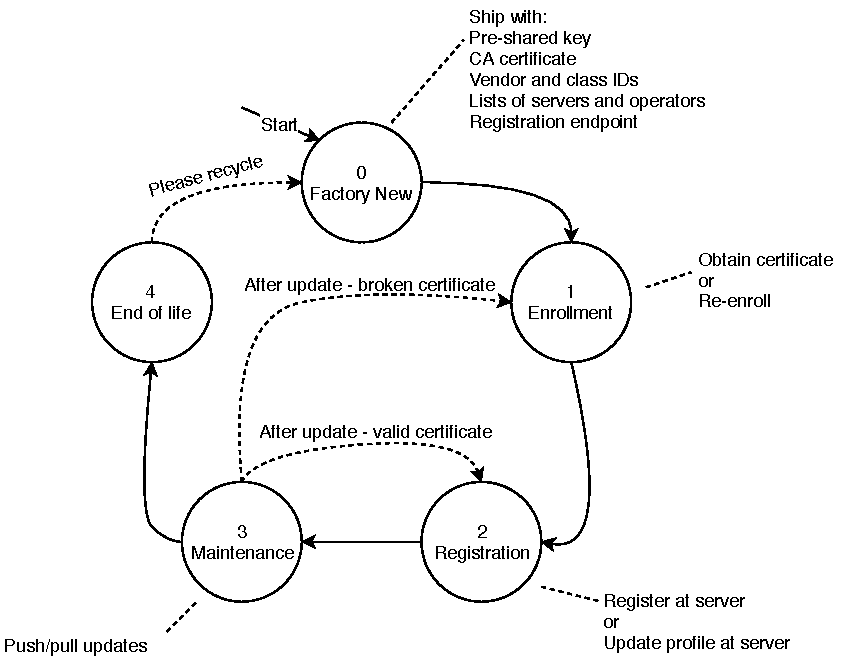
\includegraphics{images/lifecycle.pdf}
\end{figure}

Note that the life cycle does not mention authorization. Authorization tokens are far too
short lived compared to certificates and profiles to be of concern in the life cycle.
Requesting and verifying tokens would happen in the maintenance stage when a device is
being updated, but it is a level of detail too fine for the life cycle model.

\section{Predetermined Information}
\label{sec:predetermined-information}
A factory new device that is to be installed in an IoT network needs to be shipped with
some information in order to enroll and register at a server and trust future
communications. A pre-shared key and CA certificate are needed for the device to trust the
CA and for the CA to know the device is supposed to receive a certificate. The device must
be aware of its own vendor and class IDs in order to verify manifests and register at an
update server. Registration also requires a known registration endpoint, this can be a
well-known endpoint implemented by all update servers. Lastly, the device needs whitelists
of operators and update servers in order to trust traffic originating from them. Any
operator or update server that is not whitelisted is to be ignored.

\section{Enrollment and Registering}
\label{sec:enrollment-registering}
With the required information a device can enter the enrollment stage. Devices obtain
certificates by enrolling at the CA, which as previously mentioned requires a pre-shared
key and CA certificate. After obtaining a certificate the device can be trusted by the
servers and operators as well as other devices, allowing for secure communication.

The next stage is registering. By sending vendor and class IDs alongside its firmware
version to a registration endpoint, devices can register and have an update server create
a profile for them. The information in the profile tells through which protocols to reach
the device and which version it is running. This information is transient and will change
upon a successful update. Update servers must handle devices re-registering by either
updating the relevant parts of the profile or creating an entirely new one. The approach
chosen is implementation dependant.

\section{Maintenance}
\label{sec:maintenance}
After a device is enrolled and registered it enters the maintenance stage. The maintenance
stage can be expected to last for several years and this is where the device performs its
duties as well as receives and applies updates. After an update, a device will either move
back to the enrollment or registration stage. If the certificate is broken after updating,
as discussed in Section~\ref{sec:key-management}, the device moves back to the enrollment
stage to obtain a new certificate. After obtaining a new, valid certificate it can update
its profile in the registration stage. 

If the certificate is still valid after the update, there is no need to re-enroll and the
device moves directly back to the registration stage, updating the profile at the servers.
Finally the device moves to the maintenance stage once again, and so forth. The device
will remain in the maintenance stage until it either breaks or is taken out of service. If
you are a manufacturer of IoT devices please consider recycling or (securely) re-using
devices, starting the life cycle anew.

\section{Summary}
\label{sec:4-summary}
This chapter has presented a life cycle view of a device in need of updates. Understanding
the life cycle helps preparing the device for updates as well as letting it react
accordingly to being updates. To continue being operational is a security concern and
devices must be able to last for long, thus applying many updates. With a proposed
architecture and life cycle in place, the architecture can be profiled to provide
implementers help when deciding upon an implementation. Profiles are the topic of the next
chapter.

\end{document}